% !TEX TS-program = pdflatex
\documentclass[11pt]{article}

% -------------------- Packages --------------------
\usepackage[a4paper,margin=1in]{geometry}
\usepackage{amsmath,amssymb}
\usepackage[T1]{fontenc}
\usepackage{lmodern}
\usepackage{xcolor}
\usepackage{tcolorbox}
\tcbuselibrary{skins,breakable}
\usepackage{enumitem}
\usepackage{hyperref}
\usepackage{tikz}
\usetikzlibrary{calc,intersections,angles,quotes,arrows.meta}

\pagestyle{empty}

% -------------------- Dark Theme Colors --------------------
\definecolor{bg}{HTML}{000000}
\definecolor{pairbg}{HTML}{121212}
\definecolor{solbg}{HTML}{0A0A0A}
\definecolor{border}{HTML}{2A2A2A}
\definecolor{text}{HTML}{FFFFFF}
\definecolor{muted}{HTML}{C9CDD3}
\definecolor{gold}{HTML}{FFD700}
\definecolor{green}{HTML}{4ADE80}
\definecolor{cyan}{HTML}{38BDF8}

\pagecolor{bg}
\color{text}

\hypersetup{
  colorlinks=true,
  linkcolor=cyan,
  urlcolor=cyan
}

\setlength{\parindent}{0pt}
\setlength{\parskip}{10pt}

\setlist[itemize]{left=1.4em,itemsep=6pt,topsep=6pt}
\setlist[enumerate]{left=1.6em,itemsep=4pt,topsep=4pt}

% -------------------- tcolorbox Base --------------------
\tcbset{
  enhanced,
  breakable,
  arc=12pt,
  boxrule=0.8pt,
  left=16pt,right=16pt,top=12pt,bottom=12pt
}

\newtcolorbox{QAPair}[1]{%
  colback=pairbg,
  colbacklower=solbg,
  colframe=border,
  coltext=text,
  title=\textcolor{gold}{\bfseries #1},
  fonttitle=\bfseries,
  coltitle=text,
  segmentation style={draw=border, dashed, line width=0.6pt}
}

\newtcolorbox{QuickBox}{%
  colback=pairbg,
  colframe=cyan,
  coltext=text,
  fontupper=\color{text},
  borderline north={4pt}{0pt}{cyan},
  arc=14pt,
  boxrule=0.8pt
}

\newcommand{\Step}[1]{\textcolor{muted}{\textbf{Step #1:}}}
\newcommand{\StepPic}[2]{%
  \textcolor{muted}{\bfseries #1}\par
  \begin{center}
  #2
  \end{center}
}

% -------------------- TikZ styles --------------------
\tikzset{
  solidline/.style={draw=cyan, line width=0.95pt},
  dashedline/.style={draw=cyan, line width=0.9pt, dash pattern=on 3pt off 2pt},
  faint/.style={draw=muted, line width=0.7pt},
  lab/.style={text=muted, font=\small},
  pt/.style={circle, fill=cyan, draw=cyan, inner sep=1.25pt},
}

% ============================================================
\begin{document}

\begin{center}
{\LARGE\bfseries \textcolor{gold}{Exercise 10.1 --- Constructions (Solutions)}}\\[-2pt]
\end{center}

\begin{QuickBox}
{\color{cyan}\bfseries Quick construction facts}\par\medskip
\begin{itemize}
\item \textbf{Angle sum in a triangle:} $\angle A+\angle B+\angle C=180^\circ$.
\item \textbf{SAS / RHS / ASA construction idea:}
  \begin{itemize}
  \item \textbf{SAS:} draw one given side $\rightarrow$ make given angle at its endpoint $\rightarrow$ mark other given side on the ray $\rightarrow$ join.
  \item \textbf{ASA:} draw the given side between angles $\rightarrow$ construct the two given angles at the endpoints $\rightarrow$ rays meet at the third vertex.
  \item \textbf{RHS:} draw a leg $\rightarrow$ make right angle $\rightarrow$ use circle with given hypotenuse to locate the third point.
  \end{itemize}
\item \textbf{SSA (ambiguous case):} can give \textbf{0, 1, or 2} triangles (circle may cut the ray in 0/1/2 points).
\end{itemize}
\end{QuickBox}

% ============================================================
% 1(a)
\begin{QAPair}{Question 1 (a)}
\textcolor{gold}{\bfseries Question:} Construct $\triangle ABC$ when $AB=5.8$ cm, $AC=4.2$ cm, and $\angle A=90^\circ$.

\tcblower
\textcolor{green}{\bfseries Construction (with intermediate drawings):}
\[
\begin{aligned}
\Step{1}\;& \text{Draw the base }AB=5.8\text{ cm}.\\
\Step{2}\;& \text{At }A,\text{ construct a right angle and draw the ray }AX.\\
\Step{3}\;& \text{With compass radius }4.2\text{ cm and center }A,\text{ cut the ray at }C\ (AC=4.2\text{ cm}).\\
\Step{4}\;& \text{Join }BC.\ \triangle ABC\text{ is obtained.}
\end{aligned}
\]

\StepPic{Step 1 (draw $AB=5.8$ cm)}{

\begin{tikzpicture}[scale=0.9]
  \coordinate (A) at (0,0);
  \coordinate (B) at (5.8,0);
  \draw[solidline] (A)--(B);
  \node[pt] at (A) {};
  \node[pt] at (B) {};
  \node[lab,below left] at (A) {$A$};
  \node[lab,below] at (B) {$B$};
  \node[lab,below] at ($(A)!0.5!(B)$) {$5.8$ cm};
\end{tikzpicture}
}

\StepPic{Step 2 (make $\angle A=90^\circ$ and draw ray)}{
\begin{tikzpicture}[scale=0.9]
  \coordinate (A) at (0,0);
  \coordinate (B) at (5.8,0);
  \draw[solidline] (A)--(B);
  \draw[dashedline] (A)--+(0,5.0);
  % right-angle marker
  \draw[faint] (A) ++(0.7,0) -- ++(0,0.7) -- ++(-0.7,0);
  \node[pt] at (A) {};
  \node[pt] at (B) {};
  \node[lab,below left] at (A) {$A$};
  \node[lab,below] at (B) {$B$};
  \node[lab,below] at ($(A)!0.5!(B)$) {$5.8$ cm};
  \node[lab] at (1.1,1.1) {$90^\circ$};
\end{tikzpicture}
}

\StepPic{Step 3 (mark $AC=4.2$ cm using a circle arc)}{
\begin{tikzpicture}[scale=0.9]
  \coordinate (A) at (0,0);
  \coordinate (B) at (5.8,0);
  \coordinate (X) at (0,5.0);
  \coordinate (C) at (0,4.2);

  \draw[solidline] (A)--(B);
  \draw[dashedline] (A)--(X);
  \draw[dashedline] (A) circle (4.2); % compass swing

  \draw[faint] (A) ++(0.7,0) -- ++(0,0.7) -- ++(-0.7,0);

  \node[pt] at (A) {};
  \node[pt] at (B) {};
  \node[pt] at (C) {};
  \node[lab,below left] at (A) {$A$};
  \node[lab,below] at (B) {$B$};
  \node[lab,left] at (C) {$C$};
  \node[lab,below] at ($(A)!0.5!(B)$) {$5.8$ cm};
  \node[lab,left] at ($(A)!0.5!(C)$) {$4.2$ cm};
\end{tikzpicture}
}

\StepPic{Step 4 (join $BC$ to complete the triangle)}{
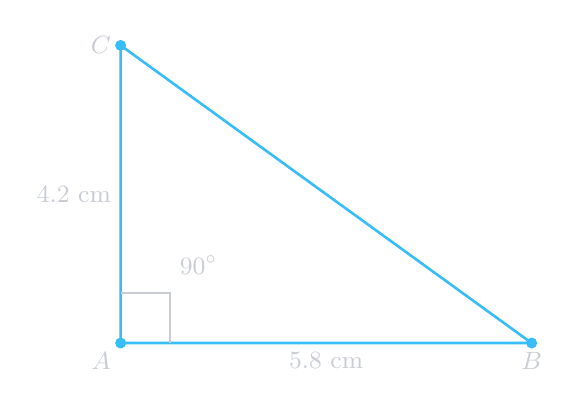
\begin{tikzpicture}[scale=0.9]
  \coordinate (A) at (0,0);
  \coordinate (B) at (5.8,0);
  \coordinate (C) at (0,4.2);

  \draw[solidline] (A)--(B)--(C)--cycle;
  \draw[faint] (A) ++(0.7,0) -- ++(0,0.7) -- ++(-0.7,0);

  \node[pt] at (A) {};
  \node[pt] at (B) {};
  \node[pt] at (C) {};
  \node[lab,below left] at (A) {$A$};
  \node[lab,below] at (B) {$B$};
  \node[lab,left] at (C) {$C$};
  \node[lab,below] at ($(A)!0.5!(B)$) {$5.8$ cm};
  \node[lab,left] at ($(A)!0.5!(C)$) {$4.2$ cm};
  \node[lab] at (1.1,1.1) {$90^\circ$};
\end{tikzpicture}
}
\end{QAPair}

% ============================================================
% 1(b)
\begin{QAPair}{Question 1 (b)}
\textcolor{gold}{\bfseries Question:} Construct $\triangle LMN$ when $LM=4$ cm, $MN=4.7$ cm, and $\angle M=120^\circ$.

\tcblower
\textcolor{green}{\bfseries Construction (with intermediate drawings):}
\[
\begin{aligned}
\Step{1}\;& \text{Draw }MN=4.7\text{ cm}.\\
\Step{2}\;& \text{At }M,\text{ construct }120^\circ\text{ and draw a ray }ML.\\
\Step{3}\;& \text{With center }M\text{ and radius }4\text{ cm, cut the ray at }L\ (ML=4\text{ cm}).\\
\Step{4}\;& \text{Join }LN.\ \triangle LMN\text{ is obtained.}
\end{aligned}
\]

\StepPic{Step 1 (draw $MN=4.7$ cm)}{

\begin{tikzpicture}[scale=0.9]
  \coordinate (M) at (0,0);
  \coordinate (N) at (4.7,0);
  \draw[solidline] (M)--(N);
  \node[pt] at (M) {};
  \node[pt] at (N) {};
  \node[lab,below left] at (M) {$M$};
  \node[lab,below] at (N) {$N$};
  \node[lab,below] at ($(M)!0.5!(N)$) {$4.7$ cm};
\end{tikzpicture}
}

\StepPic{Step 2 (make $\angle NML=120^\circ$ and draw ray)}{
\begin{tikzpicture}[scale=0.9]
  \coordinate (M) at (0,0);
  \coordinate (N) at (4.7,0);
  \draw[solidline] (M)--(N);
  \draw[dashedline] (M)--+(120:5.3);
  \draw[faint] (M) ++(1.0,0) arc (0:120:1.0);
  \node[pt] at (M) {};
  \node[pt] at (N) {};
  \node[lab,below left] at (M) {$M$};
  \node[lab,below] at (N) {$N$};
  \node[lab] at (0.95,0.6) {$120^\circ$};
\end{tikzpicture}
}

\StepPic{Step 3 (mark $ML=4$ cm using a circle arc)}{
\begin{tikzpicture}[scale=0.9]
  \coordinate (M) at (0,0);
  \coordinate (N) at (4.7,0);
  \coordinate (L) at ($(M)+(120:4)$);

  \draw[solidline] (M)--(N);
  \draw[dashedline] (M)--+(120:5.3);
  \draw[dashedline] (M) circle (4); % compass swing

  \node[pt] at (M) {};
  \node[pt] at (N) {};
  \node[pt] at (L) {};
  \node[lab,below left] at (M) {$M$};
  \node[lab,below] at (N) {$N$};
  \node[lab,above left] at (L) {$L$};
  \node[lab,below] at ($(M)!0.5!(N)$) {$4.7$ cm};
  \node[lab,left] at ($(M)!0.5!(L)$) {$4$ cm};
\end{tikzpicture}
}

\StepPic{Step 4 (join $LN$)}{
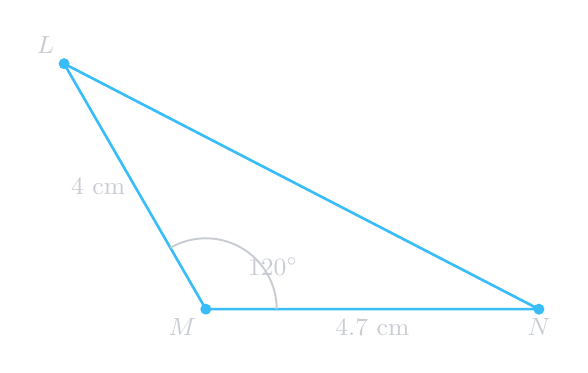
\begin{tikzpicture}[scale=0.9]
  \coordinate (M) at (0,0);
  \coordinate (N) at (4.7,0);
  \coordinate (L) at ($(M)+(120:4)$);

  \draw[solidline] (L)--(M)--(N)--cycle;

  \node[pt] at (M) {};
  \node[pt] at (N) {};
  \node[pt] at (L) {};
  \node[lab,below left] at (M) {$M$};
  \node[lab,below] at (N) {$N$};
  \node[lab,above left] at (L) {$L$};
  \node[lab,below] at ($(M)!0.5!(N)$) {$4.7$ cm};
  \node[lab,left] at ($(M)!0.5!(L)$) {$4$ cm};
  \draw[faint] (M) ++(1.0,0) arc (0:120:1.0);
  \node[lab] at (0.95,0.6) {$120^\circ$};
\end{tikzpicture}
}
\end{QAPair}
% ============================================================
% 1(c)  --- REPLACE YOUR ENTIRE Q1(c) BLOCK WITH THIS
\begin{QAPair}{Question 1 (c)}
\textcolor{gold}{\bfseries Question:} Construct $\triangle PQR$ when $PQ=7.2$ cm, $\angle P=45^\circ$, $\angle Q=75^\circ$.

\tcblower
\textcolor{green}{\bfseries Construction (ASA, with intermediate drawings):}
\[
\begin{aligned}
\Step{1}\;& \text{Draw }PQ=7.2\text{ cm}.\\
\Step{2}\;& \text{At }P,\text{ construct }45^\circ\text{ with }PQ\text{ and draw the ray }PR.\\
\Step{3}\;& \text{At }Q,\text{ construct }75^\circ\text{ with }QP\text{ and draw the ray }QR.\\
\Step{4}\;& \text{The rays meet at }R.\ \text{Join }PR\text{ and }QR.\ \triangle PQR\text{ is obtained.}
\end{aligned}
\]

\StepPic{Step 1 (Draw $PQ=7.2$ cm)}{

\begin{tikzpicture}[scale=0.90]
  \coordinate (P) at (0,0);
  \coordinate (Q) at (7.2,0);
  \draw[solidline] (P)--(Q);
  \node[pt] at (P) {};
  \node[pt] at (Q) {};
  \node[lab,below] at (P) {$P$};
  \node[lab,below] at (Q) {$Q$};
  \node[lab,below] at ($(P)!0.5!(Q)$) {$7.2$ cm};
\end{tikzpicture}
}

\StepPic{Step 2 (At $P$, make $45^\circ$ and draw ray $PR$)}{
\begin{tikzpicture}[scale=0.90]
  \coordinate (P) at (0,0);
  \coordinate (Q) at (7.2,0);

  \draw[solidline] (P)--(Q);
  \draw[dashedline] (P)--+(45:6.5); % ray PR

  % angle marker at P
  \draw[faint] (P) ++(1.0,0) arc (0:45:1.0);
  \node[lab] at ($(P)+(1.05,0.40)$) {$45^\circ$};

  \node[pt] at (P) {};
  \node[pt] at (Q) {};
  \node[lab,below] at (P) {$P$};
  \node[lab,below] at (Q) {$Q$};
  \node[lab,below] at ($(P)!0.5!(Q)$) {$7.2$ cm};
\end{tikzpicture}
}

\StepPic{Step 3 (At $Q$, make $75^\circ$ and draw ray $QR$)}{
\begin{tikzpicture}[scale=0.90]
  \coordinate (P) at (0,0);
  \coordinate (Q) at (7.2,0);

  \draw[solidline] (P)--(Q);

  % At Q, angle is 75° with QP (which points left).
  % So the ray QR goes in direction 180°-75° = 105° from positive x-axis.
  \draw[dashedline] (Q)--+(105:6.5); % ray QR

  % angle marker at Q
  \draw[faint] (Q) ++(-1.0,0) arc (180:105:1.0);
  \node[lab] at ($(Q)+(-0.85,0.55)$) {$75^\circ$};

  \node[pt] at (P) {};
  \node[pt] at (Q) {};
  \node[lab,below] at (P) {$P$};
  \node[lab,below] at (Q) {$Q$};
  \node[lab,below] at ($(P)!0.5!(Q)$) {$7.2$ cm};
\end{tikzpicture}
}

\StepPic{Step 4 (Rays meet at $R$; join to complete $\triangle PQR$)}{
\begin{tikzpicture}[scale=0.90]
  \coordinate (P) at (0,0);
  \coordinate (Q) at (7.2,0);

  % define rays as "name paths" so we can intersect them
  \path[name path=rayP] (P) -- +(45:9);
  \path[name path=rayQ] (Q) -- +(105:9);

  \path[name intersections={of=rayP and rayQ, by=R}];

  % triangle
  \draw[solidline] (P)--(Q)--(R)--cycle;

  % keep rays visible as construction lines
  \draw[dashedline] (P)--+(45:6.5);
  \draw[dashedline] (Q)--+(105:6.5);

  % angle markers
  \draw[faint] (P) ++(1.0,0) arc (0:45:1.0);
  \draw[faint] (Q) ++(-1.0,0) arc (180:105:1.0);

  \node[pt] at (P) {};
  \node[pt] at (Q) {};
  \node[pt] at (R) {};
  \node[lab,below] at (P) {$P$};
  \node[lab,below] at (Q) {$Q$};
  \node[lab,above] at (R) {$R$};

  \node[lab,below] at ($(P)!0.5!(Q)$) {$7.2$ cm};
  \node[lab] at ($(P)+(1.05,0.40)$) {$45^\circ$};
  \node[lab] at ($(Q)+(-0.85,0.55)$) {$75^\circ$};
\end{tikzpicture}
}
\end{QAPair}


% ============================================================
% 1(d)
\begin{QAPair}{Question 1 (d)}
\textcolor{gold}{\bfseries Question:} Construct $\triangle XYZ$ when $XY=5$ cm, $\angle X=30^\circ$, $\angle Z=105^\circ$.

\tcblower
\textcolor{green}{\bfseries Construction (with intermediate drawings):}

First find the third angle:
\[
\angle Y = 180^\circ-30^\circ-105^\circ=45^\circ.
\]
\[
\begin{aligned}
\Step{1}\;& \text{Draw }XY=5\text{ cm}.\\
\Step{2}\;& \text{At }X,\text{ construct }30^\circ\text{ and draw ray }XZ.\\
\Step{3}\;& \text{At }Y,\text{ construct }45^\circ\text{ and draw ray }YZ.\\
\Step{4}\;& \text{Rays meet at }Z.\text{ Join }ZX\text{ and }ZY.
\end{aligned}
\]

\StepPic{Step 1 (draw $XY=5$ cm)}{

\begin{tikzpicture}[scale=0.9]
  \coordinate (X) at (0,0);
  \coordinate (Y) at (5,0);
  \draw[solidline] (X)--(Y);
  \node[pt] at (X) {};
  \node[pt] at (Y) {};
  \node[lab,below] at (X) {$X$};
  \node[lab,below] at (Y) {$Y$};
  \node[lab,below] at ($(X)!0.5!(Y)$) {$5$ cm};
\end{tikzpicture}
}

\StepPic{Step 2 (draw ray at $X$ making $30^\circ$)}{
\begin{tikzpicture}[scale=0.9]
  \coordinate (X) at (0,0);
  \coordinate (Y) at (5,0);
  \draw[solidline] (X)--(Y);
  \draw[dashedline] (X)--+(30:6.5);
  \draw[faint] (X) ++(1.0,0) arc (0:30:1.0);
  \node[pt] at (X) {};
  \node[pt] at (Y) {};
  \node[lab,below] at (X) {$X$};
  \node[lab,below] at (Y) {$Y$};
  \node[lab] at (0.95,0.25) {$30^\circ$};
\end{tikzpicture}
}

\StepPic{Step 3 (draw ray at $Y$ making $45^\circ$)}{
\begin{tikzpicture}[scale=0.9]
  \coordinate (X) at (0,0);
  \coordinate (Y) at (5,0);
  \draw[solidline] (X)--(Y);
  % angle at Y is 45 with YX (to the left), so direction 180-45=135
  \draw[dashedline] (Y)--+(135:6.5);
  \draw[faint] (Y) ++(-1.0,0) arc (180:135:1.0);
  \node[pt] at (X) {};
  \node[pt] at (Y) {};
  \node[lab,below] at (X) {$X$};
  \node[lab,below] at (Y) {$Y$};
  \node[lab] at (4.15,0.45) {$45^\circ$};
\end{tikzpicture}
}

\StepPic{Step 4 (intersection gives $Z$; final triangle)}{
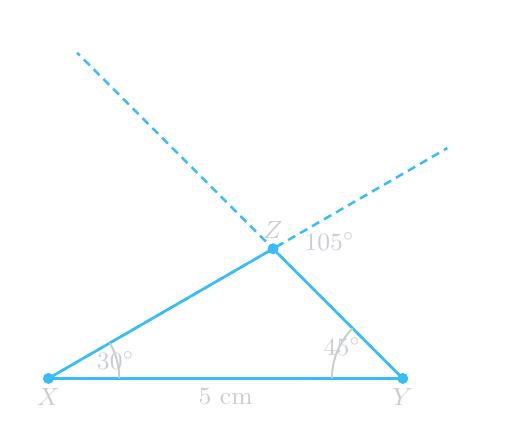
\begin{tikzpicture}[scale=0.9]
  \coordinate (X) at (0,0);
  \coordinate (Y) at (5,0);
  \path[name path=rayX] (X) -- +(30:7);
  \path[name path=rayY] (Y) -- +(135:7);
  \path[name intersections={of=rayX and rayY, by=Z}];

  \draw[solidline] (X)--(Y)--(Z)--cycle;
  \draw[dashedline] (X)--+(30:6.5);
  \draw[dashedline] (Y)--+(135:6.5);

  \draw[faint] (X) ++(1.0,0) arc (0:30:1.0);
  \draw[faint] (Y) ++(-1.0,0) arc (180:135:1.0);

  \node[pt] at (X) {};
  \node[pt] at (Y) {};
  \node[pt] at (Z) {};
  \node[lab,below] at (X) {$X$};
  \node[lab,below] at (Y) {$Y$};
  \node[lab,above] at (Z) {$Z$};
  \node[lab,below] at ($(X)!0.5!(Y)$) {$5$ cm};
  \node[lab] at (0.95,0.25) {$30^\circ$};
  \node[lab] at (4.15,0.45) {$45^\circ$};
  \node[lab] at ($(Z)+(0.8,0.1)$) {$105^\circ$};
\end{tikzpicture}
}
\end{QAPair}

% ============================================================
% 2(a)
\begin{QAPair}{Question 2 (a)}
\textcolor{gold}{\bfseries Question:} Construct $\triangle ABC$ where possible: $AB=6.8$ cm, $BC=8.1$ cm, $\angle A=90^\circ$.

\tcblower
\textcolor{green}{\bfseries Answer (Possible, RHS idea):}

\[
\begin{aligned}
\Step{1}\;& \text{Because }\angle A=90^\circ,\text{ side }BC\text{ is the hypotenuse. Since }8.1>6.8,\text{ it is possible.}\\
\Step{2}\;& \text{Draw }AB=6.8\text{ cm}.\\
\Step{3}\;& \text{At }A,\text{ erect a perpendicular ray }AX\text{ to }AB.\\
\Step{4}\;& \text{With center }B\text{ and radius }8.1\text{ cm, draw a circle/arc cutting }AX\text{ at }C.\\
\Step{5}\;& \text{Join }AC\text{ and }BC.
\end{aligned}
\]

\StepPic{Step 1 (draw $AB=6.8$ cm)}{

\begin{tikzpicture}[scale=0.85]
  \coordinate (A) at (0,0);
  \coordinate (B) at (6.8,0);
  \draw[solidline] (A)--(B);
  \node[pt] at (A) {};
  \node[pt] at (B) {};
  \node[lab,below left] at (A) {$A$};
  \node[lab,below] at (B) {$B$};
  \node[lab,below] at ($(A)!0.5!(B)$) {$6.8$ cm};
\end{tikzpicture}
}

\StepPic{Step 2 (erect perpendicular at $A$)}{
\begin{tikzpicture}[scale=0.85]
  \coordinate (A) at (0,0);
  \coordinate (B) at (6.8,0);
  \draw[solidline] (A)--(B);
  \draw[dashedline] (A)--+(0,5.5);
  \draw[faint] (A) ++(0.7,0) -- ++(0,0.7) -- ++(-0.7,0);
  \node[pt] at (A) {};
  \node[pt] at (B) {};
  \node[lab,below left] at (A) {$A$};
  \node[lab,below] at (B) {$B$};
  \node[lab] at (1.1,1.1) {$90^\circ$};
\end{tikzpicture}
}

\StepPic{Step 3 (swing radius $BC=8.1$ cm from center $B$)}{
\begin{tikzpicture}[scale=0.85]
  \coordinate (A) at (0,0);
  \coordinate (B) at (6.8,0);
  \path[name path=perpA] (A) -- +(0,6.2);
  \path[name path=circB] (B) circle (8.1);
  \path[name intersections={of=perpA and circB, by=C}];

  \draw[solidline] (A)--(B);
  \draw[dashedline] (A)--+(0,6.0);
  \draw[dashedline] (B) circle (8.1);

  \node[pt] at (A) {};
  \node[pt] at (B) {};
  \node[pt] at (C) {};
  \node[lab,below left] at (A) {$A$};
  \node[lab,below] at (B) {$B$};
  \node[lab,left] at (C) {$C$};
  \node[lab,below] at ($(A)!0.5!(B)$) {$6.8$ cm};
  \node[lab] at ($(B)+(1.6,2.6)$) {$8.1$ cm};
\end{tikzpicture}
}

\StepPic{Step 4 (join to complete triangle)}{
\begin{tikzpicture}[scale=0.85]
  \coordinate (A) at (0,0);
  \coordinate (B) at (6.8,0);
  \path[name path=perpA] (A) -- +(0,6.2);
  \path[name path=circB] (B) circle (8.1);
  \path[name intersections={of=perpA and circB, by=C}];

  \draw[solidline] (A)--(B)--(C)--cycle;
  \draw[faint] (A) ++(0.7,0) -- ++(0,0.7) -- ++(-0.7,0);

  \node[pt] at (A) {};
  \node[pt] at (B) {};
  \node[pt] at (C) {};
  \node[lab,below left] at (A) {$A$};
  \node[lab,below] at (B) {$B$};
  \node[lab,left] at (C) {$C$};
  \node[lab,below] at ($(A)!0.5!(B)$) {$6.8$ cm};
  \node[lab,right] at ($(B)!0.5!(C)$) {$8.1$ cm};
\end{tikzpicture}
}
\end{QAPair}

% ============================================================
% 2(b)
\begin{QAPair}{Question 2 (b)}
\textcolor{gold}{\bfseries Question:} Construct $\triangle DEF$ where possible: $DE=5.2$ cm, $DF=4$ cm, $\angle E=45^\circ$.

\tcblower
\textcolor{green}{\bfseries Answer (Possible; SSA may give two triangles):}
\[
\begin{aligned}
\Step{1}\;& \text{Draw }DE=5.2\text{ cm}.\\
\Step{2}\;& \text{At }E,\text{ construct }45^\circ\text{ and draw ray }EF.\\
\Step{3}\;& \text{With center }D\text{ and radius }4\text{ cm, draw a circle/arc cutting the ray.}\\
\Step{4}\;& \text{If the ray cuts the circle at }F_1\text{ and }F_2,\text{ then two triangles are possible.}\\
\Step{5}\;& \text{Join }DF_1,EF_1\text{ and }DF_2,EF_2.
\end{aligned}
\]

\StepPic{Step 1 (draw $DE=5.2$ cm)}{

\begin{tikzpicture}[scale=0.9]
  \coordinate (D) at (0,0);
  \coordinate (E) at (5.2,0);
  \draw[solidline] (D)--(E);
  \node[pt] at (D) {};
  \node[pt] at (E) {};
  \node[lab,below left] at (D) {$D$};
  \node[lab,below] at (E) {$E$};
  \node[lab,below] at ($(D)!0.5!(E)$) {$5.2$ cm};
\end{tikzpicture}
}

\StepPic{Step 2 (draw ray at $E$ making $45^\circ$ with $ED$)}{
\begin{tikzpicture}[scale=0.9]
  \coordinate (D) at (0,0);
  \coordinate (E) at (5.2,0);
  \draw[solidline] (D)--(E);
  % 45 with ED (to the left), so direction 180-45=135
  \draw[dashedline] (E)--+(135:5.8);
  \draw[faint] (E) ++(-1.0,0) arc (180:135:1.0);
  \node[pt] at (D) {};
  \node[pt] at (E) {};
  \node[lab,below left] at (D) {$D$};
  \node[lab,below] at (E) {$E$};
  \node[lab] at (4.25,0.45) {$45^\circ$};
\end{tikzpicture}
}

\StepPic{Step 3 (swing radius $DF=4$ cm from center $D$)}{
\begin{tikzpicture}[scale=0.9]
  \coordinate (D) at (0,0);
  \coordinate (E) at (5.2,0);
  \path[name path=rayE] (E) -- +(135:7);
  \path[name path=circD] (D) circle (4);
  \path[name intersections={of=rayE and circD, by={Fone,Ftwo}}];

  \draw[solidline] (D)--(E);
  \draw[dashedline] (E)--+(135:6.3);
  \draw[dashedline] (D) circle (4);

  \node[pt] at (D) {};
  \node[pt] at (E) {};
  \node[pt] at (Fone) {};
  \node[pt] at (Ftwo) {};
  \node[lab,below left] at (D) {$D$};
  \node[lab,below] at (E) {$E$};
  \node[lab,above left] at (Fone) {$F_1$};
  \node[lab,left] at (Ftwo) {$F_2$};
  \node[lab] at ($(D)+(2.1,2.7)$) {$4$ cm};
\end{tikzpicture}
}

\StepPic{Step 4 (join to show both possible triangles)}{
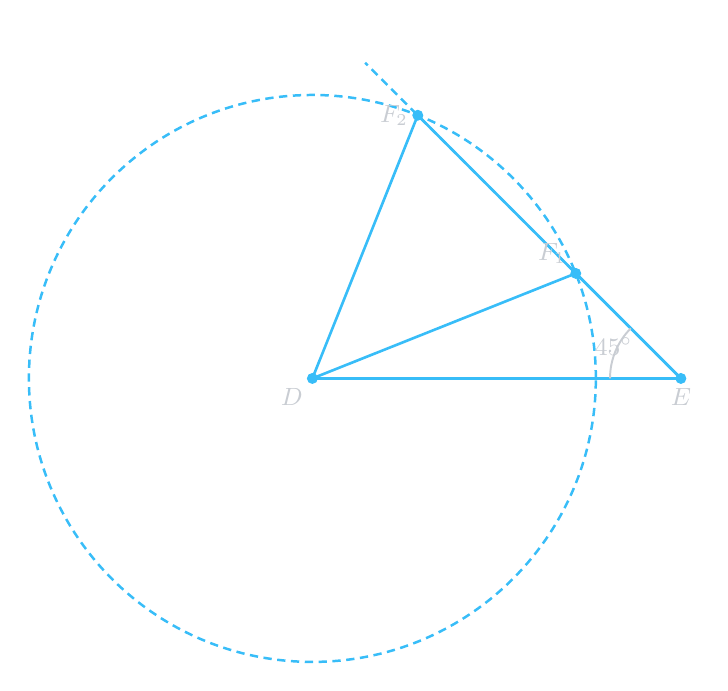
\begin{tikzpicture}[scale=0.9]
  \coordinate (D) at (0,0);
  \coordinate (E) at (5.2,0);
  \path[name path=rayE] (E) -- +(135:7);
  \path[name path=circD] (D) circle (4);
  \path[name intersections={of=rayE and circD, by={Fone,Ftwo}}];

  \draw[solidline] (D)--(E);
  \draw[solidline] (D)--(Fone)--(E);
  \draw[solidline] (D)--(Ftwo)--(E);

  \draw[dashedline] (E)--+(135:6.3);
  \draw[dashedline] (D) circle (4);
  \draw[faint] (E) ++(-1.0,0) arc (180:135:1.0);

  \node[pt] at (D) {};
  \node[pt] at (E) {};
  \node[pt] at (Fone) {};
  \node[pt] at (Ftwo) {};
  \node[lab,below left] at (D) {$D$};
  \node[lab,below] at (E) {$E$};
  \node[lab,above left] at (Fone) {$F_1$};
  \node[lab,left] at (Ftwo) {$F_2$};
  \node[lab] at (4.25,0.45) {$45^\circ$};
\end{tikzpicture}
}
\end{QAPair}

% ============================================================
% 2(c)
\begin{QAPair}{Question 2 (c)}
\textcolor{gold}{\bfseries Question:} Construct $\triangle PQR$ where possible: $QR=7.0$ cm, $PQ=5.6$ cm, $\angle R=75^\circ$.

\tcblower
\textcolor{green}{\bfseries Answer: Not possible (no intersection).}

\[
\begin{aligned}
\Step{1}\;& \text{Draw }QR=7\text{ cm}.\\
\Step{2}\;& \text{At }R,\text{ construct }75^\circ\text{ and draw a ray for }RP.\\
\Step{3}\;& \text{With center }Q\text{ and radius }5.6\text{ cm, draw a circle.}\\
\Step{4}\;& \text{If the ray does not cut the circle, then no such triangle exists.}
\end{aligned}
\]

\StepPic{Attempted construction (ray and circle do not meet)}{
\begin{tikzpicture}[scale=0.9]
  \coordinate (Q) at (0,0);
  \coordinate (R) at (7,0);

  \draw[solidline] (Q)--(R);
  \draw[dashedline] (R)--+(105:6.2); % 75 with RQ (to left) => 180-75=105
  \draw[dashedline] (Q) circle (5.6);

  \draw[faint] (R) ++(-1.0,0) arc (180:105:1.0);

  \node[pt] at (Q) {};
  \node[pt] at (R) {};
  \node[lab,below] at (Q) {$Q$};
  \node[lab,below] at (R) {$R$};
  \node[lab,below] at ($(Q)!0.5!(R)$) {$7.0$ cm};
  \node[lab] at (6.15,0.55) {$75^\circ$};

  \node[lab] at (3.5,2.2) {\textcolor{muted}{No intersection $\Rightarrow$ not possible}};
\end{tikzpicture}
}
\end{QAPair}

% ============================================================
% 2(d)
\begin{QAPair}{Question 2 (d)}
\textcolor{gold}{\bfseries Question:} Construct $\triangle XYZ$ where possible: $XY=3.8$ cm, $XZ=5$ cm, $\angle Y=60^\circ$.

\tcblower
\textcolor{green}{\bfseries Answer (Possible; with intermediate drawings):}
\[
\begin{aligned}
\Step{1}\;& \text{Draw }XY=3.8\text{ cm}.\\
\Step{2}\;& \text{At }Y,\text{ construct }60^\circ\text{ and draw ray }YZ.\\
\Step{3}\;& \text{With center }X\text{ and radius }5\text{ cm, cut the ray at }Z.\\
\Step{4}\;& \text{Join }XZ\text{ and }YZ.
\end{aligned}
\]

\StepPic{Step 1 (draw $XY=3.8$ cm)}{

\begin{tikzpicture}[scale=0.95]
  \coordinate (X) at (0,0);
  \coordinate (Y) at (3.8,0);
  \draw[solidline] (X)--(Y);
  \node[pt] at (X) {};
  \node[pt] at (Y) {};
  \node[lab,below left] at (X) {$X$};
  \node[lab,below] at (Y) {$Y$};
  \node[lab,below] at ($(X)!0.5!(Y)$) {$3.8$ cm};
\end{tikzpicture}
}

\StepPic{Step 2 (draw ray at $Y$ making $60^\circ$)}{
\begin{tikzpicture}[scale=0.95]
  \coordinate (X) at (0,0);
  \coordinate (Y) at (3.8,0);
  \draw[solidline] (X)--(Y);
  % 60 with YX (to left) => direction 180-60=120
  \draw[dashedline] (Y)--+(120:6.2);
  \draw[faint] (Y) ++(-1.0,0) arc (180:120:1.0);
  \node[pt] at (X) {};
  \node[pt] at (Y) {};
  \node[lab,below left] at (X) {$X$};
  \node[lab,below] at (Y) {$Y$};
  \node[lab] at (3.05,0.55) {$60^\circ$};
\end{tikzpicture}
}

\StepPic{Step 3 (swing radius $XZ=5$ cm from center $X$)}{
\begin{tikzpicture}[scale=0.95]
  \coordinate (X) at (0,0);
  \coordinate (Y) at (3.8,0);
  \path[name path=rayY] (Y) -- +(120:7);
  \path[name path=circX] (X) circle (5);
  \path[name intersections={of=rayY and circX, by=Z}];

  \draw[solidline] (X)--(Y);
  \draw[dashedline] (Y)--+(120:6.2);
  \draw[dashedline] (X) circle (5);

  \node[pt] at (X) {};
  \node[pt] at (Y) {};
  \node[pt] at (Z) {};
  \node[lab,below left] at (X) {$X$};
  \node[lab,below] at (Y) {$Y$};
  \node[lab,left] at (Z) {$Z$};
  \node[lab,left] at ($(X)!0.5!(Z)$) {$5$ cm};
\end{tikzpicture}
}

\StepPic{Step 4 (join to complete triangle)}{
\begin{tikzpicture}[scale=0.95]
  \coordinate (X) at (0,0);
  \coordinate (Y) at (3.8,0);
  \path[name path=rayY] (Y) -- +(120:7);
  \path[name path=circX] (X) circle (5);
  \path[name intersections={of=rayY and circX, by=Z}];

  \draw[solidline] (X)--(Y)--(Z)--cycle;

  \draw[faint] (Y) ++(-1.0,0) arc (180:120:1.0);

  \node[pt] at (X) {};
  \node[pt] at (Y) {};
  \node[pt] at (Z) {};
  \node[lab,below left] at (X) {$X$};
  \node[lab,below] at (Y) {$Y$};
  \node[lab,left] at (Z) {$Z$};
  \node[lab,below] at ($(X)!0.5!(Y)$) {$3.8$ cm};
  \node[lab,left] at ($(X)!0.5!(Z)$) {$5$ cm};
  \node[lab] at (3.05,0.55) {$60^\circ$};
\end{tikzpicture}
}
\end{QAPair}

% ============================================================
% 2(e)
\begin{QAPair}{Question 2 (e)}
\textcolor{gold}{\bfseries Question:} Two sides are $5.7$ cm and $7.5$ cm, and angle $105^\circ$ is opposite the side $7.5$ cm. Construct the triangle (where possible).

\tcblower
\textcolor{green}{\bfseries Answer (Possible, unique; with intermediate drawings):}

Let $AB=5.7$ cm, $\angle A=105^\circ$, and $BC=7.5$ cm (so $BC$ is opposite $\angle A$).

\[
\begin{aligned}
\Step{1}\;& \text{Draw }AB=5.7\text{ cm}.\\
\Step{2}\;& \text{At }A,\text{ construct }105^\circ\text{ and draw ray }AC.\\
\Step{3}\;& \text{With center }B\text{ and radius }7.5\text{ cm, cut the ray at }C.\\
\Step{4}\;& \text{Join }BC.
\end{aligned}
\]

\StepPic{Step 1 (draw $AB=5.7$ cm)}{

\begin{tikzpicture}[scale=0.85]
  \coordinate (A) at (0,0);
  \coordinate (B) at (5.7,0);
  \draw[solidline] (A)--(B);
  \node[pt] at (A) {};
  \node[pt] at (B) {};
  \node[lab,below left] at (A) {$A$};
  \node[lab,below] at (B) {$B$};
  \node[lab,below] at ($(A)!0.5!(B)$) {$5.7$ cm};
\end{tikzpicture}
}

\StepPic{Step 2 (draw ray at $A$ making $105^\circ$)}{
\begin{tikzpicture}[scale=0.85]
  \coordinate (A) at (0,0);
  \coordinate (B) at (5.7,0);
  \draw[solidline] (A)--(B);
  \draw[dashedline] (A)--+(105:6.8);
  \draw[faint] (A) ++(1.0,0) arc (0:105:1.0);
  \node[pt] at (A) {};
  \node[pt] at (B) {};
  \node[lab,below left] at (A) {$A$};
  \node[lab,below] at (B) {$B$};
  \node[lab] at (0.75,0.95) {$105^\circ$};
\end{tikzpicture}
}

\StepPic{Step 3 (swing radius $BC=7.5$ cm from center $B$)}{
\begin{tikzpicture}[scale=0.85]
  \coordinate (A) at (0,0);
  \coordinate (B) at (5.7,0);
  \path[name path=rayA] (A) -- +(105:8);
  \path[name path=circB] (B) circle (7.5);
  \path[name intersections={of=rayA and circB, by=C}];

  \draw[solidline] (A)--(B);
  \draw[dashedline] (A)--+(105:7.2);
  \draw[dashedline] (B) circle (7.5);

  \node[pt] at (A) {};
  \node[pt] at (B) {};
  \node[pt] at (C) {};
  \node[lab,below left] at (A) {$A$};
  \node[lab,below] at (B) {$B$};
  \node[lab,left] at (C) {$C$};
  \node[lab] at ($(B)+(1.7,2.6)$) {$7.5$ cm};
\end{tikzpicture}
}

\StepPic{Step 4 (join $BC$ to complete)}{
\begin{tikzpicture}[scale=0.85]
  \coordinate (A) at (0,0);
  \coordinate (B) at (5.7,0);
  \path[name path=rayA] (A) -- +(105:8);
  \path[name path=circB] (B) circle (7.5);
  \path[name intersections={of=rayA and circB, by=C}];

  \draw[solidline] (A)--(B)--(C)--cycle;
  \draw[faint] (A) ++(1.0,0) arc (0:105:1.0);

  \node[pt] at (A) {};
  \node[pt] at (B) {};
  \node[pt] at (C) {};
  \node[lab,below left] at (A) {$A$};
  \node[lab,below] at (B) {$B$};
  \node[lab,left] at (C) {$C$};
  \node[lab,below] at ($(A)!0.5!(B)$) {$5.7$ cm};
  \node[lab,right] at ($(B)!0.5!(C)$) {$7.5$ cm};
  \node[lab] at (0.75,0.95) {$105^\circ$};
\end{tikzpicture}
}
\end{QAPair}

% ============================================================
% 2(f)
\begin{QAPair}{Question 2 (f)}
\textcolor{gold}{\bfseries Question:} Two sides are $6.1$ cm and $3.8$ cm, and angle $30^\circ$ is opposite the side $3.8$ cm. Construct the triangle (where possible).

\tcblower
\textcolor{green}{\bfseries Answer (Possible; SSA may give two triangles):}

Let $AB=6.1$ cm, $\angle A=30^\circ$, and $BC=3.8$ cm (so $BC$ is opposite $\angle A$).

\[
\begin{aligned}
\Step{1}\;& \text{Draw }AB=6.1\text{ cm}.\\
\Step{2}\;& \text{At }A,\text{ construct }30^\circ\text{ and draw ray }AC.\\
\Step{3}\;& \text{With center }B\text{ and radius }3.8\text{ cm, draw a circle cutting the ray at }C_1,C_2.\\
\Step{4}\;& \text{Join }BC_1,AC_1\text{ and }BC_2,AC_2\text{ (two possible triangles).}
\end{aligned}
\]

\StepPic{Step 1 (draw $AB=6.1$ cm)}{

\begin{tikzpicture}[scale=0.9]
  \coordinate (A) at (0,0);
  \coordinate (B) at (6.1,0);
  \draw[solidline] (A)--(B);
  \node[pt] at (A) {};
  \node[pt] at (B) {};
  \node[lab,below left] at (A) {$A$};
  \node[lab,below] at (B) {$B$};
  \node[lab,below] at ($(A)!0.5!(B)$) {$6.1$ cm};
\end{tikzpicture}
}

\StepPic{Step 2 (draw ray at $A$ making $30^\circ$)}{
\begin{tikzpicture}[scale=0.9]
  \coordinate (A) at (0,0);
  \coordinate (B) at (6.1,0);
  \draw[solidline] (A)--(B);
  \draw[dashedline] (A)--+(30:8.0);
  \draw[faint] (A) ++(1.0,0) arc (0:30:1.0);
  \node[pt] at (A) {};
  \node[pt] at (B) {};
  \node[lab,below left] at (A) {$A$};
  \node[lab,below] at (B) {$B$};
  \node[lab] at (0.95,0.25) {$30^\circ$};
\end{tikzpicture}
}

\StepPic{Step 3 (swing radius $BC=3.8$ cm from center $B$)}{
\begin{tikzpicture}[scale=0.9]
  \coordinate (A) at (0,0);
  \coordinate (B) at (6.1,0);
  \path[name path=rayA] (A) -- +(30:10);
  \path[name path=circB] (B) circle (3.8);
  \path[name intersections={of=rayA and circB, by={Cone,Ctwo}}];

  \draw[solidline] (A)--(B);
  \draw[dashedline] (A)--+(30:9.2);
  \draw[dashedline] (B) circle (3.8);

  \node[pt] at (A) {};
  \node[pt] at (B) {};
  \node[pt] at (Cone) {};
  \node[pt] at (Ctwo) {};
  \node[lab,below left] at (A) {$A$};
  \node[lab,below] at (B) {$B$};
  \node[lab,above] at (Cone) {$C_1$};
  \node[lab,above right] at (Ctwo) {$C_2$};
  \node[lab] at ($(B)+(1.4,1.7)$) {$3.8$ cm};
\end{tikzpicture}
}

\StepPic{Step 4 (join to show both possible triangles)}{
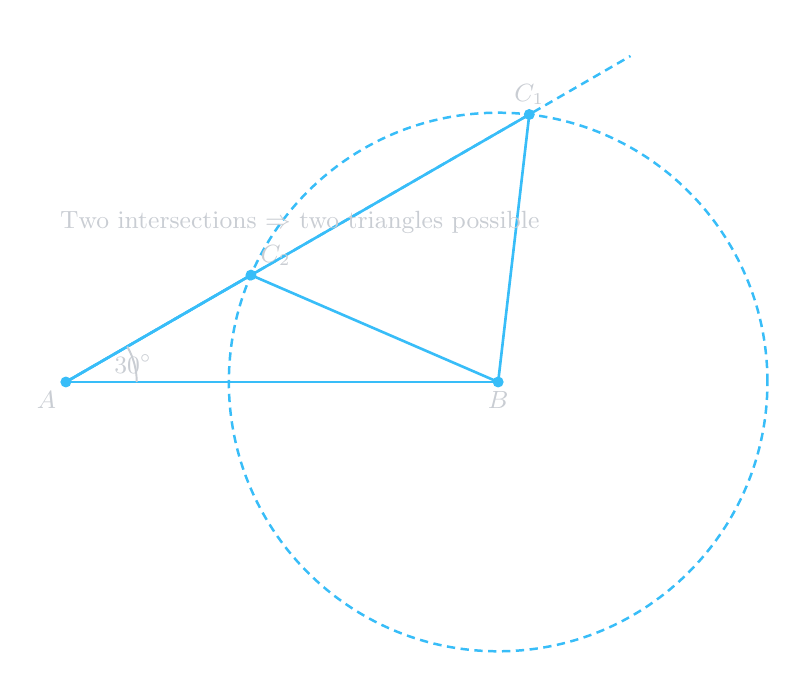
\begin{tikzpicture}[scale=0.9]
  \coordinate (A) at (0,0);
  \coordinate (B) at (6.1,0);
  \path[name path=rayA] (A) -- +(30:10);
  \path[name path=circB] (B) circle (3.8);
  \path[name intersections={of=rayA and circB, by={Cone,Ctwo}}];

  \draw[solidline] (A)--(B);
  \draw[solidline] (A)--(Cone)--(B);
  \draw[solidline] (A)--(Ctwo)--(B);

  \draw[dashedline] (A)--+(30:9.2);
  \draw[dashedline] (B) circle (3.8);
  \draw[faint] (A) ++(1.0,0) arc (0:30:1.0);

  \node[pt] at (A) {};
  \node[pt] at (B) {};
  \node[pt] at (Cone) {};
  \node[pt] at (Ctwo) {};
  \node[lab,below left] at (A) {$A$};
  \node[lab,below] at (B) {$B$};
  \node[lab,above] at (Cone) {$C_1$};
  \node[lab,above right] at (Ctwo) {$C_2$};
  \node[lab] at (0.95,0.25) {$30^\circ$};

  \node[lab] at (3.3,2.25) {\textcolor{muted}{Two intersections $\Rightarrow$ two triangles possible}};
\end{tikzpicture}
}
\end{QAPair}

\end{document}
